\documentclass[12pt]{article}
\usepackage{eurosym}
\usepackage{times}
%\usepackage[T1]{fontenc}
\usepackage[bitstream-charter]{mathdesign}
\usepackage{natbib}
\usepackage{pdflscape}
\usepackage{afterpage}
\usepackage{textcomp}
\usepackage{amsmath}
\usepackage{dcolumn}
\usepackage{graphicx}
\usepackage{textcomp}
\usepackage{url}
\usepackage{xcolor}
\usepackage[colorlinks=true,citecolor=red!50!black,urlcolor=blue!50!black,linkcolor=red!50!black]{hyperref}
\setlength{\parindent}{10mm}
\usepackage[left=1in,top=1.25in,right=1.5in,bottom=1.25in]{geometry}
\usepackage{setspace}
\usepackage{sectsty}
\usepackage[title]{appendix}
\usepackage{multicol}
\usepackage{enumerate}
%\renewcommand{\footnotesize}{\normalsize}
%\sectionfont{\normalsize}
%\subsectionfont{\normalsize}
%\setlength{\footnotesep}{0.6cm}

\title{The Modern Gatekeepers in Mass Media}

\author{Patrick Kraft\\PhD. Student\\Stony Brook University \and Yanna Krupnikov\\Assistant Professor\\Stony Brook University \and Kerri Milita\\Assistant Professor\\Illinois State University \and John Barry Ryan\\Assistant Professor\\Stony Brook University}

\begin{document}
\maketitle\thispagestyle{empty}

%150 word abstract
\begin{abstract}
The abstract goes here.
\end{abstract}

\bigskip
Prepared for presentation at the annual meeting of the Midwest Political Science Association, Chicago, April 8, 2016. The manuscript and code are available on GitHub: \url{https://github.com/pwkraft/nyt}.

\newpage
\clearpage
\setcounter{page}{1}
\begin{doublespace}
\section{Introduction}
Few people have direct experiences with political events.  Rather, people's experiences with most of the important political events are mediated. People read about these events in news stories, watch these events on video and hear about the first-hand experiences of the select-few who may have participated in the events through social media. As a result, much of what people believe and know about politics is a function of mediated perceptions. Politics is often, as Walter Lippmann \citeyearpar{Lippmann1922} suggested, the ``pictures in our heads."

In recent decades, people have more and more information to choose from in order to form the political pictures in their heads. The sheer number of media carrying political information have increased. Moreover, while print and television were constrained by available space and time, the use of the internet has provided news organizations with an unprecedented capacity to produce information that is largely unconstrained by either factor. This increasing availability of information in the universe has made questions of informational choice all the more important. Given that people can choose to read information about a myriad of topics, which topics draw the most attention? Moreover, which topics do people believe others should follow?

Questions about the types of political information that people find important are not new to political science scholarship. Previous scholarship has attempted to track perceptions of importance by considering the types of stories that people are most likely to read \citep[e.g.,][]{LauRedlawsk2006}, as well as the types of stories media elites are most likely to feature prominently in media outlets \citep[e.g.,][]{Boydstun2014}. This previous research sets an important foundation, but it is a limited approach. Studies that analyze people's news choices often do so in highly controlled settings, where the universe of news options is distinctly smaller than the universe of options people encounter in their daily lives. Studies that focus on media elites offer a broader perspective, but it is one that hinges on the idea that media elites are highly attuned to the perceptions of ordinary individuals.

In this manuscript we analyze how people interact with the news using an approach that is unlike previous work on this topic. We do so by leveraging the idea that modern media provide people with the ability to reveal their news preferences. If people find something interesting and important, they are more likely to interact with the information: they may click on it, share it via social media or email the information to another person.  Analyzing these types of behaviors, in turn, provides an overview of the types of information that people believe is -- at the very least -- worthy of additional attention.

In what follows we analyze a data set that tracks the most shared and viewed stories from the New York Times.  Not only do we analyze the most shared stories, be we compare these stories to those that were not shared or read as frequently. In total, we analyze the text of 5504 unique New York Times articles.  Our analyses rely on topic models which allows us to directly compare articles. In doing so, we consider what differentiates five types of articles: (1) articles that are most viewed, (2) articles that receive the most Facebook shares, (3) articles that are most shared on Twitter, (4) articles that are most shared via email, and (5) articles that do not receive this level of attention.

The analyses presented in this manuscript are exploratory.   To this end, the results that follow present an overview of the different approaches and comparisons we can make using our dataset. Across all analyses we focus on patterns of topics, including over time changes in the types of topics that get the most attention and the structural contents of these articles.

\section{The More Things Change...}

With technology, it is very tempting to herald the era following every advancement as fundamentally different from the era that proceeded it. The reality, however, is more nuanced than that. From the invention of the printing press to television to streaming services, each new technology has allowed creative people to tell their stories to a wider audience. Still, while each medium has its subtle differences in how it tells stories, there is something fundamental about drama and comedy that remains unchanged. That is what allows modern people to enjoy stories dating all the way back to ancient Greece and even before.

There is a similar tendency among some to say that social media has transformed how we consume political information. While their clearly some differences, we would argue it is foolish to assume the old theories no longer apply. Social media allows communication with larger numbers of people in dispersed locations--including people who have never been in the same room. At the same time, despite these differences, communication via social media is still, at its heart, one person sending messages to another person. In this fundamental way, it is no different from talking at a very large table.

To examine how much has changed in the era of Facebook and Twitter, we can examine how the "two-step flow" of information is different now. In the most basic form, the two-step flow would suggest that most people receive information from their friends, family, and co-workers who pay attention to the news media \citep{Katz1957}. If this were different, then we would expect that more people got their news from the primary sources--e.g., newspapers, television news, or internet news sites. If anything has changed, fewer people are receiving information directly from these news outlets necessitating the two-step flow of information even more \citep{Prior2005}.

With off-line social networks, there is often a tendency towards political homophily with people forming and maintaining friendships with people have similar preferences \citep{Finifter1974,NoelNyhan2011}.  While it is unlikely that many people choose their discussion partners solely on the basis of politics \citep{EvelandKleinman2013}, people do associate with individuals who are similar in terms of race, religion, education, and other factors which often correlate with political affiliations \citep{McPhersonSmithLovinCook2001}. Despite the tendency toward homophily, the complex patterns of social relations allows people to hold opinions different from some of their acquaintances \citep{HuckfeldtJohnsonSprague2004}. In fact, the more one talks about politics, the more likely they are to encounter disagreement \citep{HuckfeldtMendez2008}. This means that 21st century on-line social networks, which tend towards homophily but allow for some cross-cutting exposure, are not that different from the pre-internet social networks \citep{BakshyMessingAdamic2015,Barbera2015}.

On-line social networks are larger than off-line social networks, but it is unclear how this difference matters. To describe some of the "friends" on social media as "weak" ties would stretch the definition of the concept. Granovetter \citeyearpar{Granovetter1973} noted that weak ties can provide information unavailable among an individual's intimate associates. Only a bold individual would ask for a job based on a Facebook post from someone he or she met a few times five years ago. Further, the most influential ties are those with some intimacy \citep{Kenny1998}. That is, the most important ties are those with whom one has a feeling of closeness. This feeling is more important than frequency of discussion or the duration of the connection \citep{MardsenCampbell1984}. Hence, researchers suggest individuals should not look at the entire on-line social network if one wants to understand the truly influential connections. Rather, the meaningful social network is made of the individuals with whom one has direct communication--e.g., they comment on each other's photos \citep{Jonesetal2013}.

Finally, the most politically engaged are the most likely to share political information on social media \citep{BekafigoMcBride2013}. The most politically engaged are also the most likely to discuss politics \citep{Huckfeldt2001}. The motivations in both instances are quite similar. As Ahn, Huckfeldt, and Ryan write \citeyearpar{AhnHuckfeldtRyan2014}, "We cannot expect opinion leaders to provide information that is balance, objective, and value free" (255). Opinion leaders discuss politics and post information about it on social media because they care about politics and they want to influence people. This is the most important way that the social communication is unchanged even with the internet. The modern two-step flow, like the two-step flow of previous eras, operates because individuals want to influence how people think about politics.


\section{Endogenous Agenda Setting}

To the extent that social media changes communication, it is not about interactions among peers. The major change involves how the news media interacts with the politically engaged members of the public. Whether referring to the news media as agenda setters or gatekeepers, the major theories of information flow in the 20th Century assumed that the media were the first movers in deciding what issues were important \citep{IyengarKinder1987}. Obviously, this view was always a bit oversimplified--as the "two-step flow" implies, the politically engaged members of the public acted as a second gatekeeper in regards to what stories most people heard. Further, 20th century editors would choose stories in part based on what stories they thought would sell newspapers \citep{Napoli1997}. For this reason, Thorson and Wells \citeyearpar{ThorsonWells2015} argue that we should think of modern gatekeeping in terms of "curated flows": journalists select certain stories to post on a website, engaged members select a subset of those to read, and they share an even smaller subset.

Social media adds another wrinkle to this agenda setting story. While 20th Century journalists had to anticipate which stories attract public attention and then receive noisy signals about the stories did capture the public, 21st Century journalists are able to quantify just how much attention a story is receiving. They then act on this information as they decide which stories to write about and which stories to feature \citep{TandocVosND}. In this way, modern agenda setting is endogenous. Media gatekeepers set the agenda for the engaged members of the public. Engaged members of the public act as gatekeepers for everybody else sharing certain stories and not other. The media then writes more stories about the topics the engaged members of the public are sharing.

When engaged members of the public having greater say over the agenda, this has the potential to fundamentally change the news that makes the agenda. The most basic difference comes from the beliefs of the different agenda setting actors. In journalism, there are norms that encourage journalists to be neutral and, with some notable exceptions, many view their main role as informing the public \citep{Bennett1996}. The modern engaged public is marked by extreme positions \citep{Abramowitz2010} and their main goal is to persuade \citep{AhnHuckfeldtRyan2014}. This would suggest that there will be biases in terms of what stories are passed along. Typically, we think about biases in social communication as selective sharing of information in order to make one's own party look better \citep{AhnRyan2015,PietrykaND}. The more important biases in this case, however, may result from simply which types of stories receive attention.

Hence, this new form of agenda setting has many potential implications and in this paper we will explore many issues related to this topic. We also ask a simple question: are the types of stories the news media values different from the types of stories that its readers share with others? This is the first question that any investigation in endogenous agenda setting must address. If the news media and the engaged public believe the same stories are important, then the feedback journalists receive now provides no new information to them. On the other hand, if the engaged public differs from journalists in its beliefs about what is important, then stories that would have previously been buried may begin to receive front page attention now that the journalists are more likely to follow the public.


\section{Data}

The data for this study was collected from the website of \textit{The New York Times} between February 18 and April 28, 2015. We created a macro using Visual Basic that performed an exhaustive scrape of key areas of the website.\footnote{Standard web scraping platforms and programs (e.g., Outwit, rvest) were unable to extract all of the requested information, as the three subsections intermittently experienced html changes, such as an alteration in the font size or heading classification for a particular article.  Changes such as this will cause traditional web scraping programs to skip over these articles. Thus, it was necessary to write a macro that was customized to these three subsections of \textit{The New York Times} website. Using html parsing, we documented the source code for each subsection and noted common changes to the html over a course of three days. For instance, if a text-only article is replaced on the following day by one with embedded video, the source code will change to reflect that. The macro was programmed to run every 12 hours and to export the scraped material to an excel file with three tabs (one for each subsection). Every time the macro ran, it created an additional excel file (e.g., NYT01, NYT02, etc.).} The macro consisted of three web scrapers that extracted article title, author, date, time, and URL for (1) the front page of \textit{The New York Times}, which mirrors the lead stories on the hard copy of the newspaper, (2) the digital front page, which contains more stories than the hard copy of the front page, and (3) a subset of the front page that lists the top ten most viewed, most emailed, most shared articles.

This data collection allows us to analyze every story that appeared on the hardcopy and digital front pages of the \textit{New York Times}. It also allows us to see which types of stories the journalists see as more important--those that make the front page or receive a prominent placement on the digital front page. It also allows us to separate the agenda of the engaged public into separate categories in a way that is not capable with off-line social network research. We can see the stories they believe are important--those that make the most viewed list--and separate those stories from the stories they believe are the most important for other people to know--the most share on Facebook, Twitter, or via email.

After scraping the content of all \textit{New York Times} articles for the given time frame, we created a reduced dataset where each unique article is included as a single observation. Articles that appeared several times in the original raw collection (e.g. most tweeted article for several days) or through different channels (e.g. most tweeted and most viewed) were therefore combined in a single observation. Overall, the reduced dataset contains 5504 \textit{unique} articles for subsequent analyses. For each observation, we created a vector of dichotomous variables indicating whether the respective article was included in each of the categories (most emailed, most shared on Facebook, etc.) at least once. These variables represent the matrix of covariates that will be used to model differences in topical prevalence in the collection of documents.


\section{Distribution of Topics in New York Times Articles}

We rely on a structural topic model to extract and summarize differences in content between the articles. After some preliminary analyses, we decided to estimate a total of 20 topics using the \texttt{stm} package in \texttt{R} \citep[using spectral initialization, see][]{roberts2014structural,roberts2014stm}. The total number was set such that single topics do not represent mixtures of broad news categories (such as national and international politics). While reducing the number of topics creates some important overlaps within topics, the substantial results discussed below are robust for varying model specifications. In order for the estimation to be computationally more tractable, we removed terms from the dictionary that only appeared in 10 articles or less. Figure~\ref{fig:words} presents an overview of the extracted topics by displaying words that are highly associated with the respective topic (i.e. words that have highest probabilities to appear in a given topic, see \citealt{roberts2014stm} for more details).

\begin{figure}[ht]
\caption{Highest probability words for each topic}\label{fig:words}
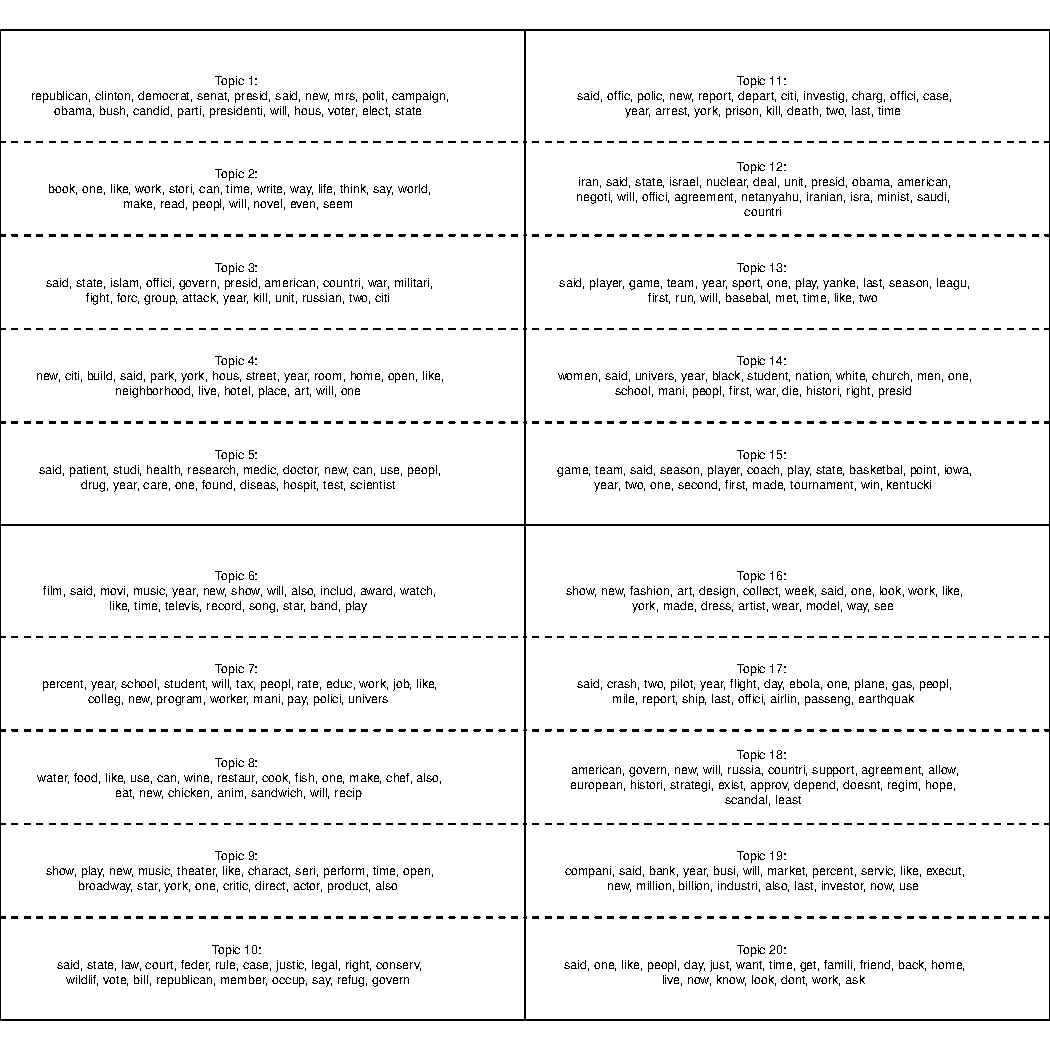
\includegraphics[width=\textwidth]{../calc/fig/words}
\end{figure}

The high probability words provide a good intuition for the topics extracted from the corpus. For example, the first topic clearly covers the US Presidential race and national politics. Topic 3, on the other hand, is mostly focused on (international) conflicts. After closely investigating the high probability words and reviewing sample articles that were estimated to be most associated with each of the topics, we decided to give them the following descriptive labels:

\begin{enumerate}\singlespacing
\begin{multicols}{2}
\item Presidential Race \item Books \item Conflicts \item Cities  \item Health
\item Movies \item Education/Inequality \item Food \item Theater \item Legal/Court
\columnbreak
\item Police \item Iran/Israel \item Baseball \item Religion \item Basketball
\item Fashion \item Natural Disaster \item International/Opinion \item Economy \item Family
\end{multicols}
\end{enumerate}

As a next step, we want to investigate the overall prevalence of each topic in the collection of \textit{New York Times} articles. Figure~\ref{fig:prop} displays the expected topic proportions in the corpus.

\begin{figure}
\caption{Expected Topic Proportions}\label{fig:prop}
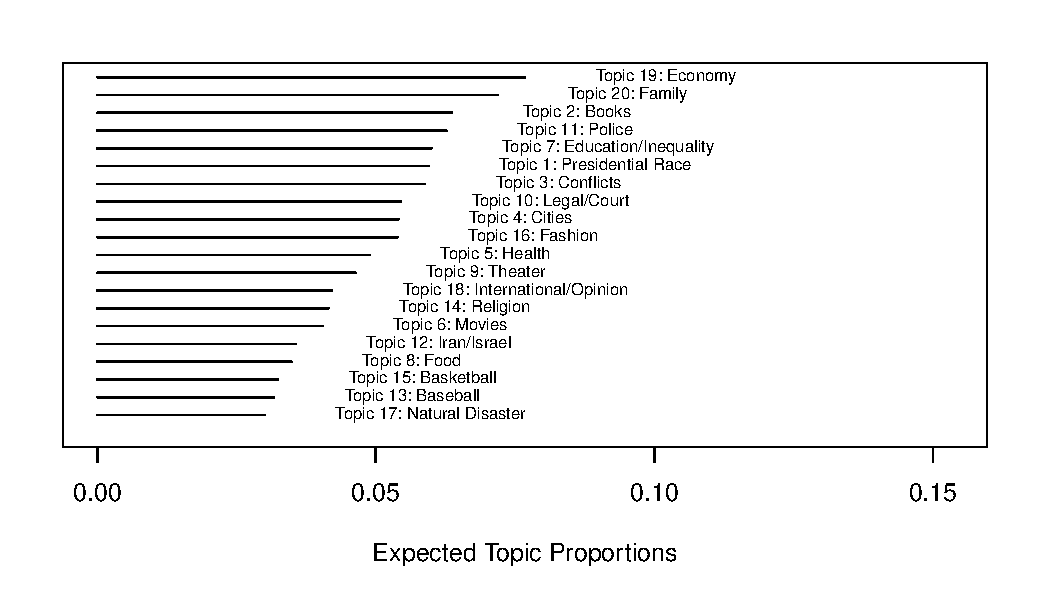
\includegraphics[width=\textwidth]{../calc/fig/prop}
\end{figure}

Interestingly, the prevalence of topics is relatively evenly distributed. Most common topics among all articles include the economy, family, books, and reports about police behavior. Less common, on the other hand, are articles that cover food, basketball, baseball, or natural disasters. However, it should be kept in mind, that each observation in the document matrix can represent multiple instances of an article in the raw collection. The proportions presented here only describe the proportions in unique articles but does not take into account how often each of the articles was included originally (e.g. as most tweeted, or most viewed multiple over a longer period of time).

Unsurprisingly, many of the topics extracted here clearly do not cover issues of political relevance. We will restrict our subsequent analyses to a subset of topics that are connected to political issues and/or actors. More specifically, we label the following topics as belonging to the broader category of Political/Economy:

\begin{enumerate}[(a)]\singlespacing
\begin{multicols}{2}
\item Presidential Race \item Conflicts \item Education/Inequality \item Legal/Court
\columnbreak
\item Police \item Iran/Israel \item International/Opinion \item Economy
\end{multicols}
\end{enumerate}

We can also directly compare how certain words differentiate between topics in order to provide additional face validity of the topic model. Consider for example topic 1 (presidential race) and topic 3 (conflicts). Figure~\ref{fig:perspectives} displays how certain words are related to each of these topics. The size of the words is proportional to the frequency of occurence in the text, and the position on the x-axis describes whether the word is more related to either of the topics.

\begin{figure}
\caption{Example for Topic Perspectives}\label{fig:perspectives}
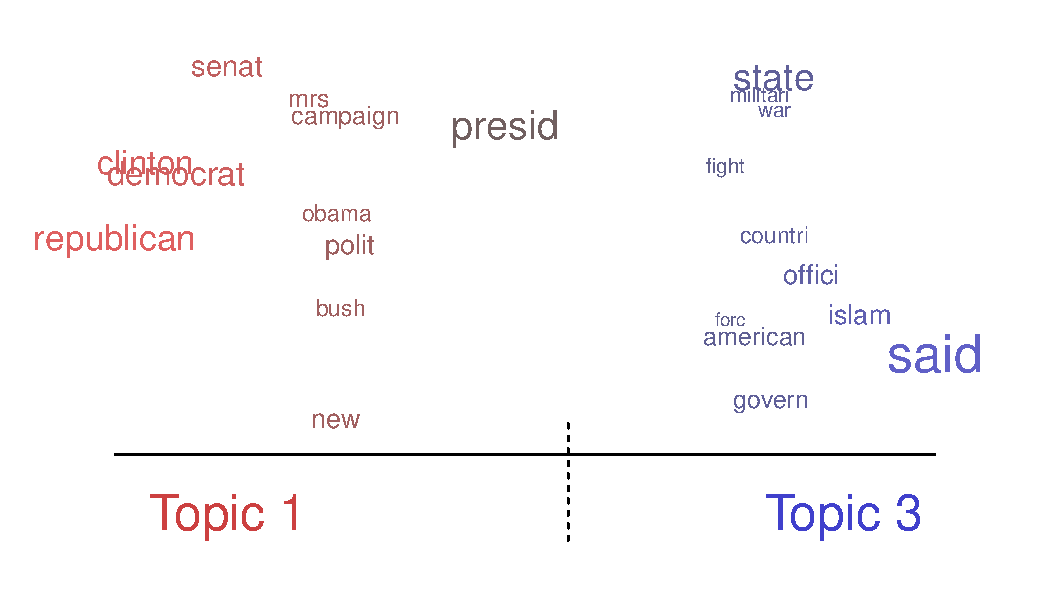
\includegraphics[width=\textwidth]{../calc/fig/perspective}
\end{figure}

In this example, we can see that ``Clinton'' and ``Republican'' is clearly associated with topic 1 (presidential race), rather than topic 3 (conflicts). The term ``president'' on the other hand, is mentioned frequently in both topics, but cannot be uniquely ascribed to either of the topics, which seems plausible.


\section{Differences in Topic Proportions between Categories}
\subsection{The \textit{Times} Agenda}
As described in \citet{roberts2014structural}, the structural topic model not only extracts topics from a collection of documents but also allows us to directly model the prevalence of topics in specific documents based on a matrix of meta-covariates. While it is also possible to use covariates in order to model differences in words used to describe certain topics, we only focus on differences with regard to \textit{how much} a topic is discussed in specific articles. The following figures display the change in the expected proportion to discuss individual topics for articles that were included in each of the categories or not. Note that we restrict our analyses on topics belonging to the category of Political/Economy. However, results for the complete set of topics are displayed in Appendix~\ref{app:res}.

As a first step, we examine the change in topic distributions for content offered by the New York Times through different channels (printed front page vs. digital sections). The results are displayed in Figure~\ref{fig:res_nyt_polecon}.

\begin{figure}
\caption{Changes in Topic Distributions (Newspaper Section)}\label{fig:res_nyt_polecon}
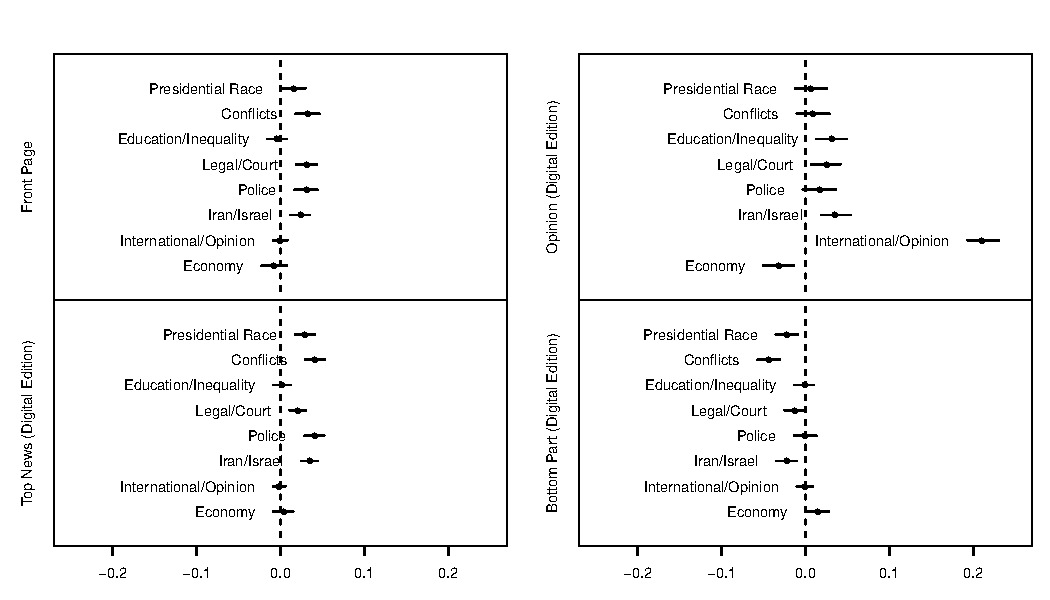
\includegraphics[width=\textwidth]{../calc/fig/res_nyt_polecon}
\end{figure}

Looking at the articles that appeared on the printed front page, we can see that the topics ``Conflicts'' and ``Legal/Court'', and ``Police'' are more likely to appear. The proportion of articles focusing on both topics is almost 5 percentage points lower than in articles that do not appear on the printed front page. Furthermore, none of the topics included here are substantially less likely to appear on the printed front page, which implies that the covers mostly topics that belong in the Political/Economy category rather than the remaining topics. Again, this result seems very plausible given our priors about the printed edition of the \textit{New York Times}.

We recover essentially the same pattern when looking at the top news section of the digital edition. The only subtle difference is that articles about the Presidential race are slightly more likely to appear on the digital front page, while articles belonging to the topic of Legal/Court are slightly less likely. The bottom section of the digital edition almost reverses the topic distribution in the top news section. Here, the proportion of articles related to the Presidential race, conflicts, and Iran/Israel are less likely to appear. Overall, instead of focusing on topics related to politics and the economy, articles on the bottom part of the digital edition cover the remaining non-political issues.

Lastly, there is a remarkable finding regarding the topic distribution in the digital opinion section. Here, we find much higher proportions for the topic labelled ``International/Opinion''. While most of the articles related to this topic cover international issues, it should be noted that many of them are opinion pieces focusing on various issues. As such, it appears that the structural topic model extracted op-eds as a unique topic category due to systematic differences in word usage. We do not view this finding to be problematic but rather as an additional validation of the structural topic model approach, since opinion pieces clearly differ in writing style and specific word choice.


\subsection{The Agenda on Social Media}

\begin{figure}
\caption{Changes in Topic Distributions (Shared/Viewed)}\label{fig:res_share_polecon}
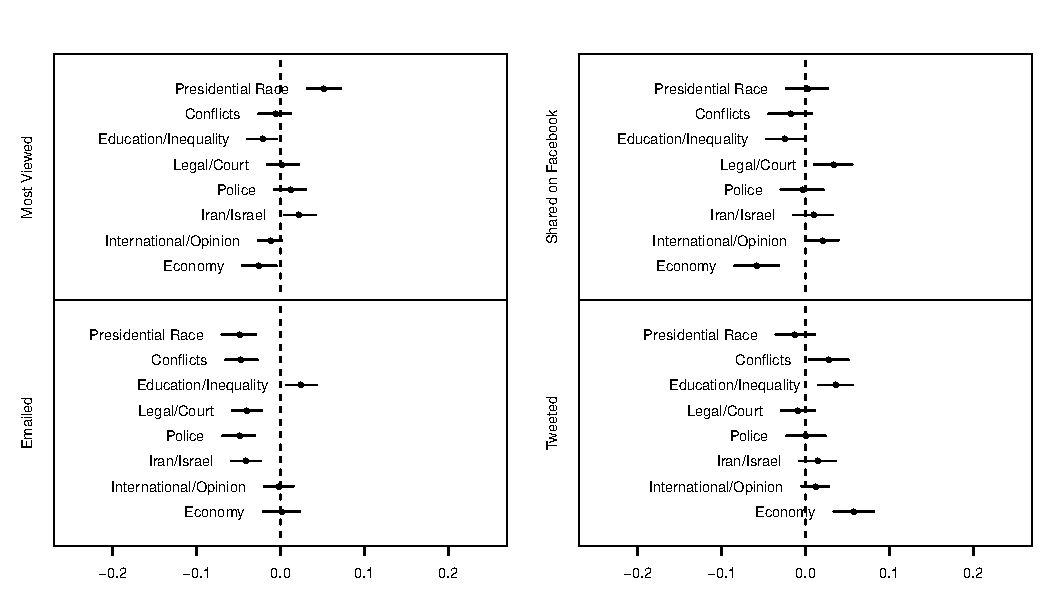
\includegraphics[width=\textwidth]{../calc/fig/res_share_polecon}
\end{figure}


Next, we compare changes in topic distributions among articles that were most shared on different platforms. Figure~\ref{fig:res_share_polecon} reveals several interesting patterns. For example, we can see that articles that were most emailed were more likely to belong to the ``Education/Inequality'' topic but less likely to belong to many of the remaining political topics such as ``Presidential Race'', ``Conflicts'', or ``Legal/Court''. On the other hand, articles that were top shared on Facebook were more likely to belong to the topic ``Supreme Court/Legal'', and ``International/Opinion''. Many articles in this topic discussed same-sex marriage and related Supreme Court decisions. As such, individuals who shared news content on Facebook were more likely to share articles related to marriage equality. Articles shared most on Twitter, on the other hand, were more likely to discuss topics of ``Economy'', ``Education/Inequality'', and ``Conflicts''.

As such, there appear to be systematic differences between users who share content through different channels. This result is plausible if we consider the underlying demographics of the average individuals using each medium. For example, people who share articles via email might be older than individuals who use social media platforms to share content. If we additionally take into account non-political issues, we see that most emailed articles have the biggest increase in the probability to belong to the topics of ``Health'' and ``Food''. On Facebook, on the other hand, users who share content are likely to be younger and therefore more interested in topics like same-sex marriage. Furthermore, sharing content rather than emailing an article to an acquaintance has the additional function of signalling political preferences to a broader audience. Articles shared on Twitter are more likely to belong to the topic ``Economy'', which could be explained by the fact that many articles in this topic address new technologies.

However, one of the most important questions is how these patterns actually translate into views? The top left part of the Figure~\ref{fig:res_share_polecon} displays change in topic proportions for articles that were most viewed. Interestingly, we observe substantial differences between the topic proportions in most viewed articles as compared to content that was shared. Articles in this category were more likely to discuss the presidential race, even though articles in this topic were not more likely to be shared on any platform. Other topics that were more likely in the most-viewed category are ``Police'' and ``Iran/Israel''. Interestingly, multiple topics that were more likely to appear in shared articles were, in fact, less likely to be most viewed (e.g. Economy on Twitter, International/Opinion on Facebook, and Education/Inequality via email). While it would be interesting to directly examine how shared articles affect traffic to the contents hosted by the \textit{New York Times}, this indirect finding is at least suggestive of the fact that attention on social media is not the most decisive factor that influences article views.


\section{Over Time Changes in the \textit{Times} and Shared Stories}
As a next step, we want to examine how the proportion of topics in each of the categories changes over time. Based on the topic model discussed above, we matched the estimated topic proportions for each article with the articles' dates of appearance. For these simplicity, we decided to focus on three main topics related to domestic politics: Presidential Race, Legal/Court, Police. However, results for the full set of political issues are displayed in Appendix~\ref{app:series}.

\begin{figure}
\caption{Topic Proportions over Time (Newspaper Section)}\label{fig:series_nyt_main}
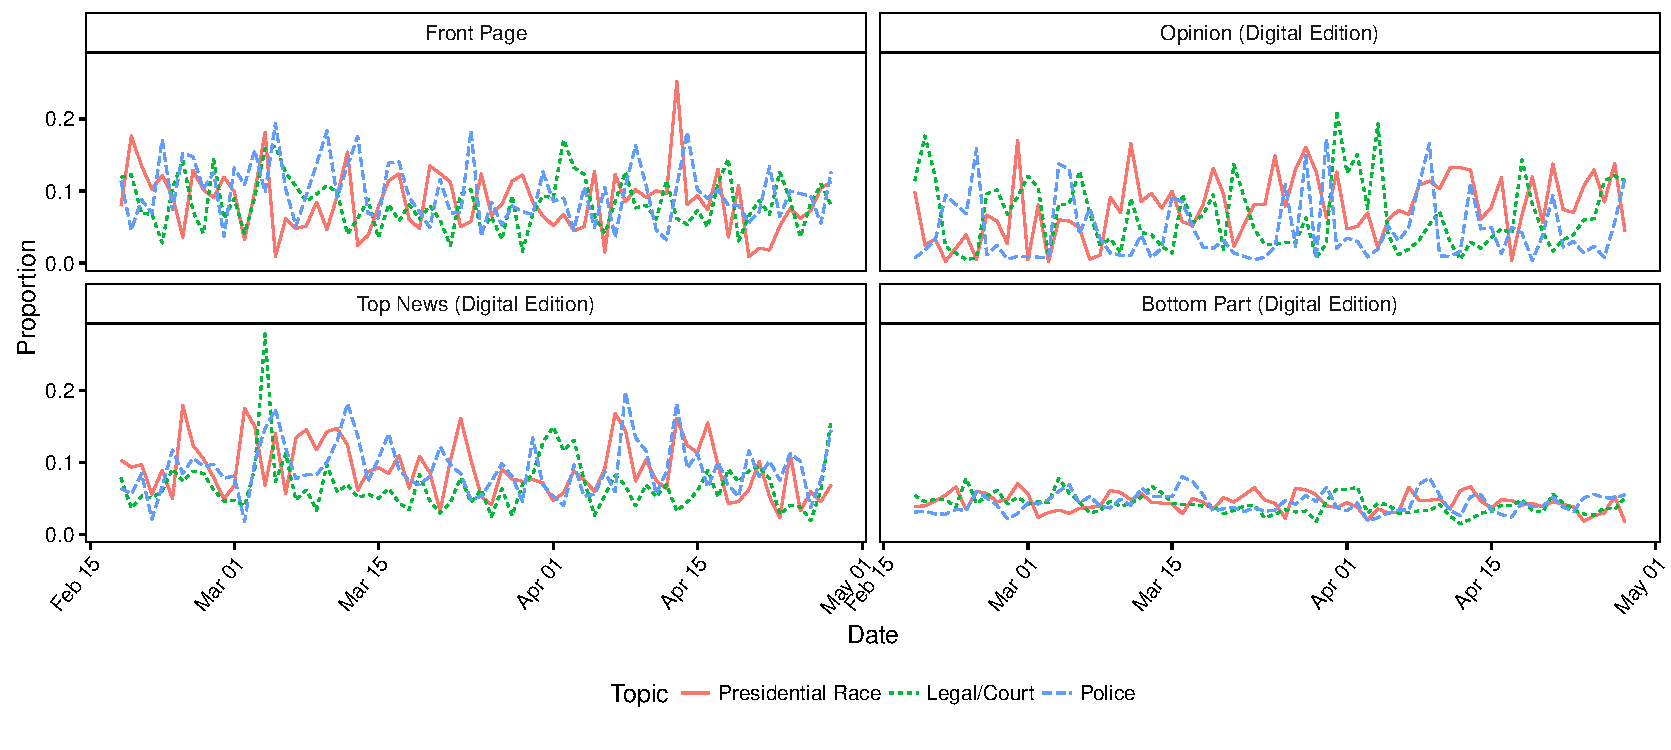
\includegraphics[width=\textwidth]{../calc/fig/series_nyt_main}
\end{figure}

Figure~\ref{fig:series_nyt_main} displays the aggregate topic proportions for in each of the \textit{New York Times} sections from mid February until end of April. Overall there is a substantial amount of variability in the relative prevalence of the three topics under consideration here. Especially the peaks in topic proportions are interesting. For example, we see that the proportion of articles related to the topic ``Legal/Court'' in the top news category spike in the beginning of March, which coincides with the overturning of Nebraska's ban on same-sex marriage by District Judge Joseph F. Batallion, as well as the Alabama Supreme Court's decision to disallow marriage licenses for same sex couples. On the printed front page, we observe a spike in the prevalence of articles related to the presidential race around April 12, which coincides with Hillary Clinton's formal announcement of her candidacy for the presidential nomination of the Democratic party. Spikes in prevalence of articles related to the police are less pronounced. However, they also appear to co-occur with events such as the shooting of Walter Scott in North Charleston, South Carolina on April 4. Overall, the results therefore show that we can recover interesting shifts in news attention based on changes in the prevalence of the recovered from the articles.

\begin{figure}
\caption{Topic Proportions over Time (Shared/Viewed)}\label{fig:series_share_main}
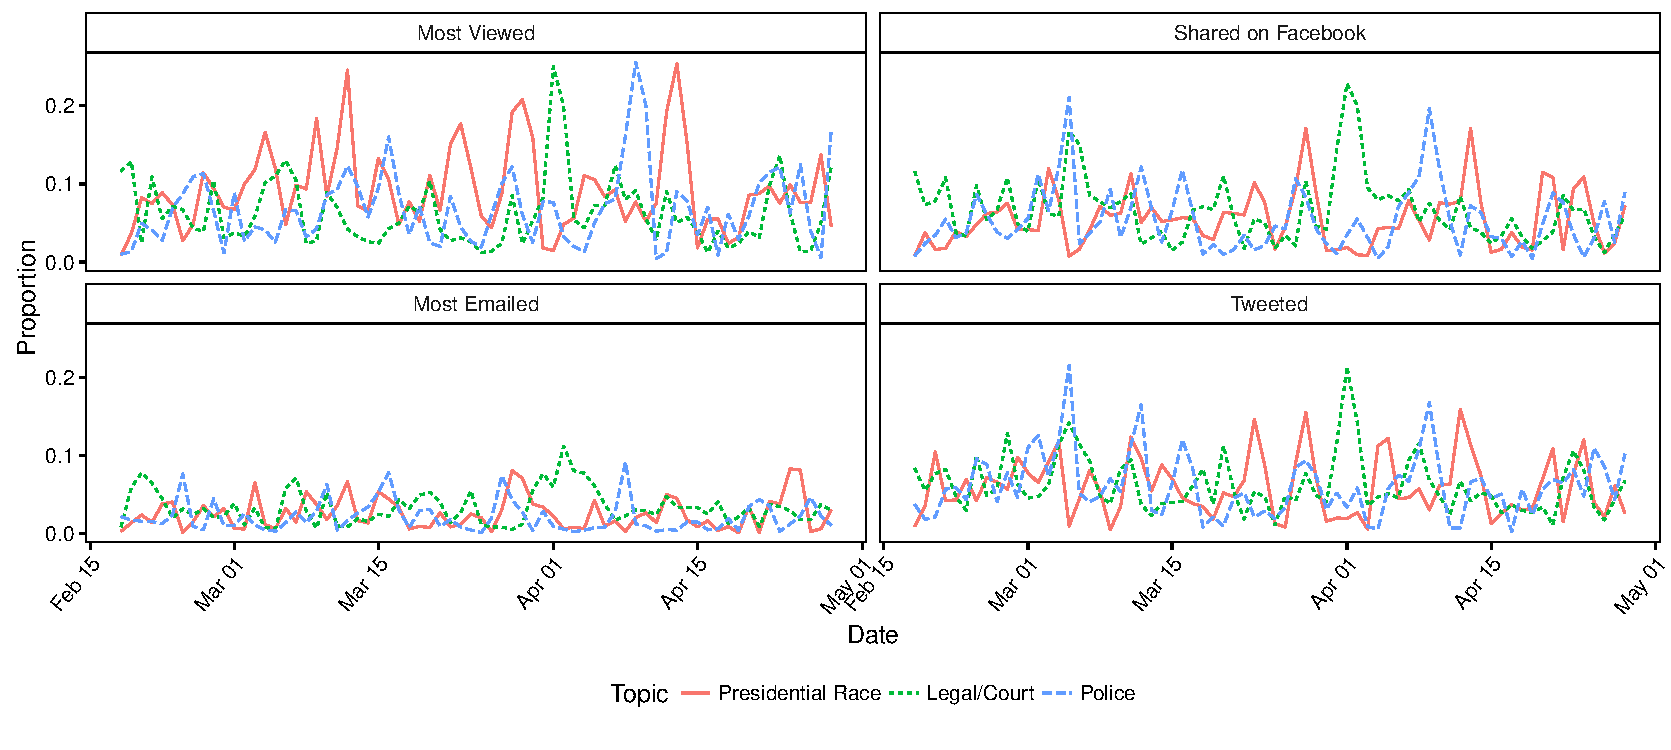
\includegraphics[width=\textwidth]{../calc/fig/series_share_main}
\end{figure}

Turning now to the articles that were most viewed and shared in Figure~\ref{fig:series_share_main}, we can identify several time points were the presidential race, court decisions, as well as the police behavior was more salient than other topics. Again, we observe heightened attention for the presidential race when Hillary Clinton anounced here candidacy, and for police behavior around the time of Walter Scott's death. Interestingly, regarding same sex marriage, there is a pronounced spike in attention around April 1, which was less strong when looking at the prevalence in each section of the newspaper. Furthermore, there is a lot more attention to the presidential race in the most viewed category than in the remaining categories, which is consistent with the previous results regarding different topic proportions.


\section{Article Readability}

Another interesting question is whether there are structural differences between articles that determine the likelihood to be shared or most viewed etc. In order to examine whether the article complexity has any effect, we calculated the Flesch-Kincaid Readability score for all articles belonging to the broader topic of Political/Economy (alternative readbility indices, like the ARI produce equivalent results). The following figure displays the mean Flesch-Kincaid scores for each article category. The score is supposed to map onto US grade years, so higher numbers indicate higher levels of difficulty.

\begin{figure}
\caption{Article Readability by Category}\label{fig:readability}
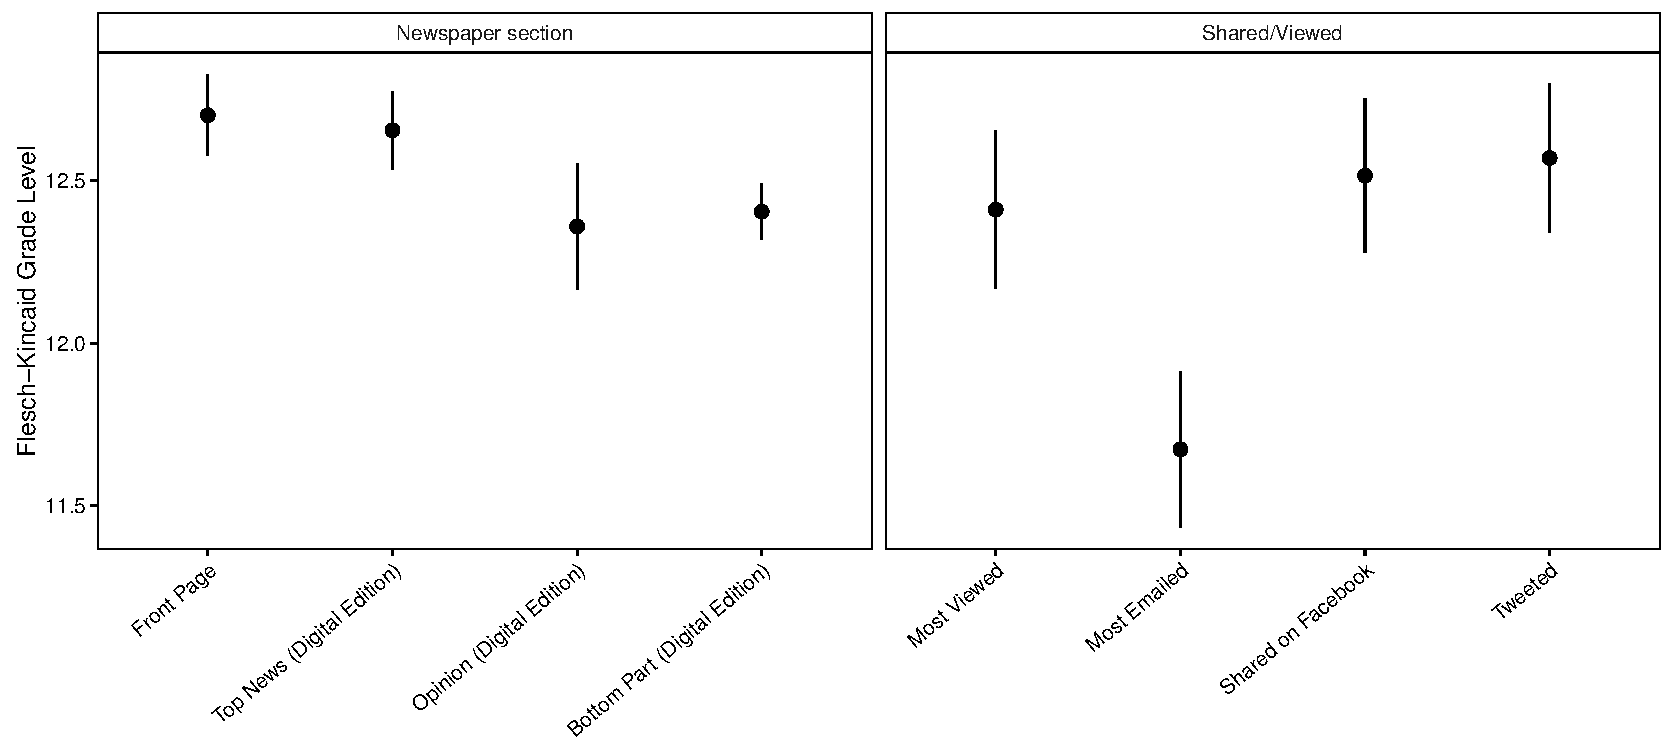
\includegraphics[width=\textwidth]{../calc/fig/readability}
\end{figure}

We find that articles on the front page as well as the digital top news section appear to be slightly more complex or harder to read than articles in the remaining categories. Furthermore, articles that were most emailed are on average less complex than articles in any of the remaining categories.


\section{What stays in the loop}

As a last step, we started examining the order in which articles appear in each of the categories discussed so far. For example, it could be interesting to see whether articles are first shared and then become most viewed (or vice versa), or whether articles are potentially moved to the top news section after being shared a lot etc. In order to get a first impression of these possible patterns, we selected all articles that were included in the dataset for mutiple days and calculated the proportion of article categories for each day since the first publication (most shared, top news etc.). Figure~\ref{fig:switch} displays the results.

\begin{figure}
\caption{What stays in the loop}\label{fig:switch}
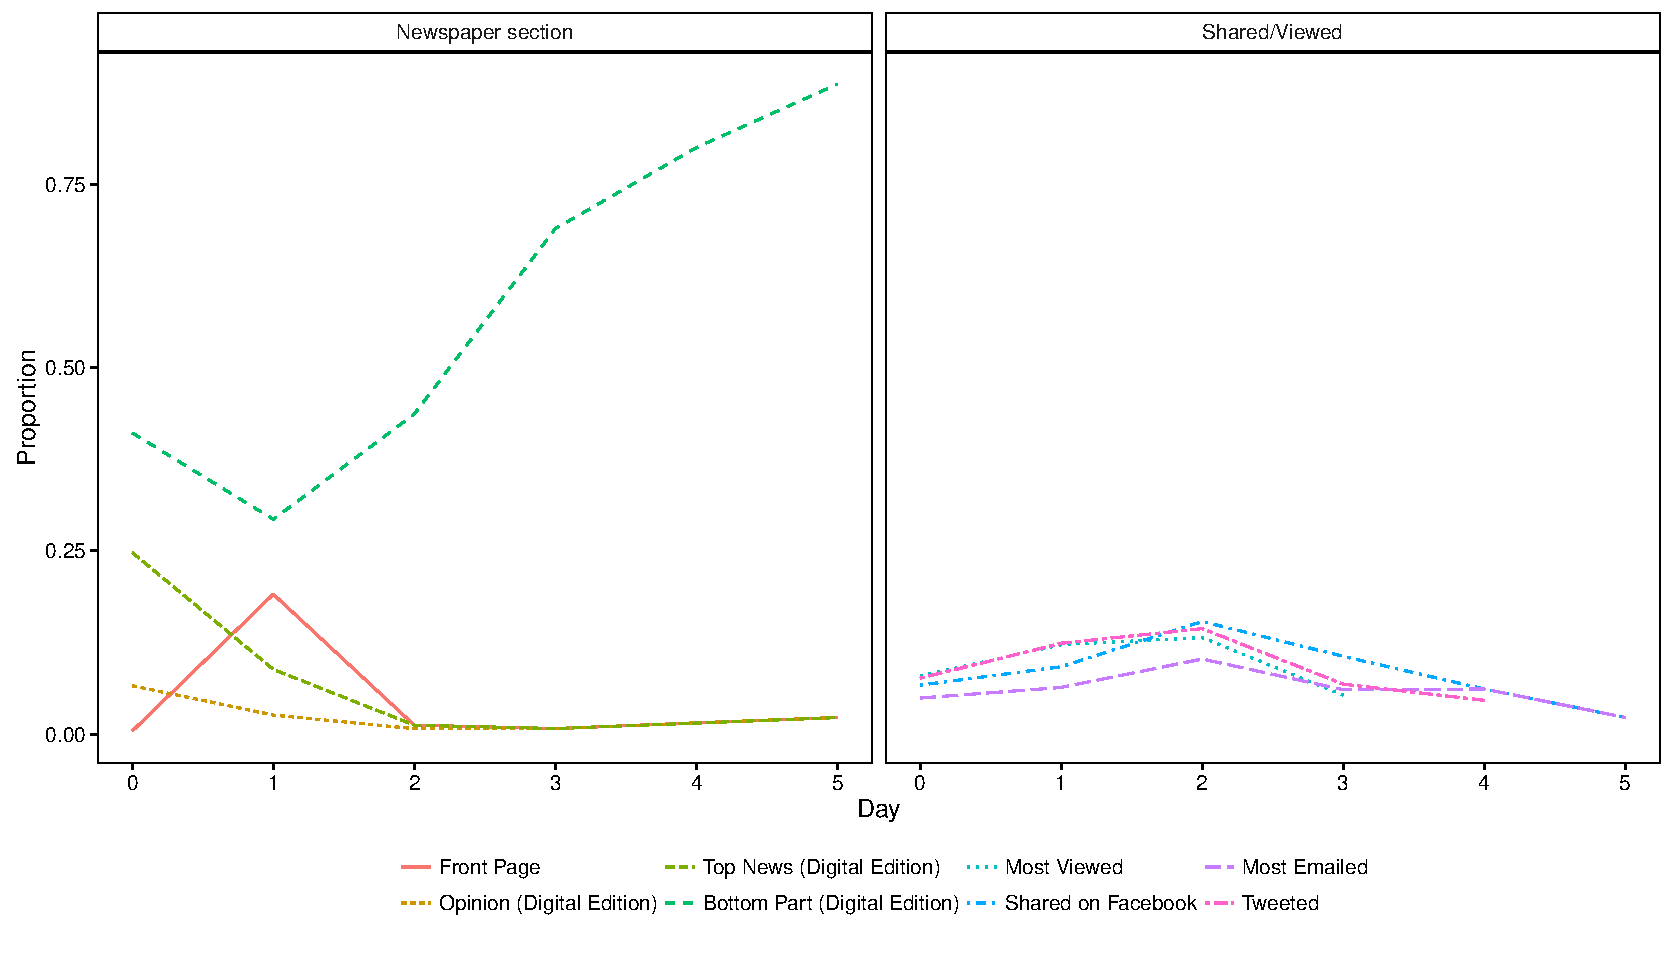
\includegraphics[width=\textwidth]{../calc/fig/switch}
\end{figure}

On the first day of publication, most articles only appeared in the bottom section of the digital edition (about 40\%), or the top news section (about 25\%). Almost none of the articles that appear in the dataset for multiple times have been published on the printed front page first. Rather, they appear in print the day after being available online, as can be seen by the increase in the proportion of front page articles at day 1 (and the respective decrease in digital articles). The proportion of articles belonging to the most shared or most viewed categories increase throughout the first three days. While the differences are not very large, it appears that articles fall into the categories most tweeted and most viewed earlier than in the categories most emailed or most shared on Facebook. Sharing on Twitter and views might therefore precede subsequent sharing on Facebook and via email. However, it is worth noting that these differences are relatively small and are so far only examined on an aggregate level. Nevertheless, these are interesting patterns that could be investigated further.


\section{Conclusion}

In this manuscript we conduct exploratory analyses tracking patterns in article sharing in the New York Times over a two-month period in 2015.  Our goal is to consider patterns in the types of articles that gain the most attention. Our findings suggest that there are differences in the types of articles that are shared across media, but more importantly there are differences in sharing patterns and the types of articles that the New York Times places on its front page. In general, if we use front-page placement as an indictor of the stories the New York Times believes are important and sharing patterns as indicators of what people find important, then we see some disagreement on importance of certain news stories.

Our results are not without limitation. First, readers of the New York Times may be different than readers of other news sources. New York Times readers, for example, are somewhat more liberal, although the left-leanings of the New York Times readers are not as extreme as the right-leanings of the Fox viewers \citep{GolbeckHansen2014}. Second, it is also possible that the perceptions of importance are contextual -- people believe articles are more important because other people have already determined that they have a level of importance. Nonetheless, if this was the only pattern driving the findings, we would have likely observed more homogeneity across all shared articles.

Finally, it is also possible that the use of the New York Times exaggerates the difference between articles that are deemed important by the newspaper�s editorial team and those shared by the public. The Times is an established brand, and as a result may be less concerned about keeping readers entertained at all times than a newspaper that is experienced more financial difficulties.  Put another way, it is possible that we would have observed more synergy between editorial choices and public behavior had we focused on a smaller newspaper's website.

Given that these initial analyses are exploratory, our goal is to conduct additional analyses that consider this data in greater depth. In particular, future steps will consider the role of additional article factors, including length.  Moreover, our next steps also additional investigation of the over-time components of this data and the temporal development of these articles.  Our goal is to track how long articles remain popular in a given cycle, which in turn will reinforce the comparisons we can make between editorial and public decisions when it comes to the importance of news.




\clearpage
\bibliographystyle{apsr2006}
\bibliography{JBRReferences.bib}


\end{doublespace}

\clearpage
\footnotesize\singlespacing
\appendices

\section{Topic Proportions between categories (all topics)}\label{app:res}
\renewcommand\thefigure{\thesection.\arabic{figure}}
\renewcommand\thetable{\thesection.\arabic{table}}
\setcounter{figure}{0}
\setcounter{table}{0}

\begin{figure}[h]
\caption{Differences between categories}\label{fig:res_nyt}
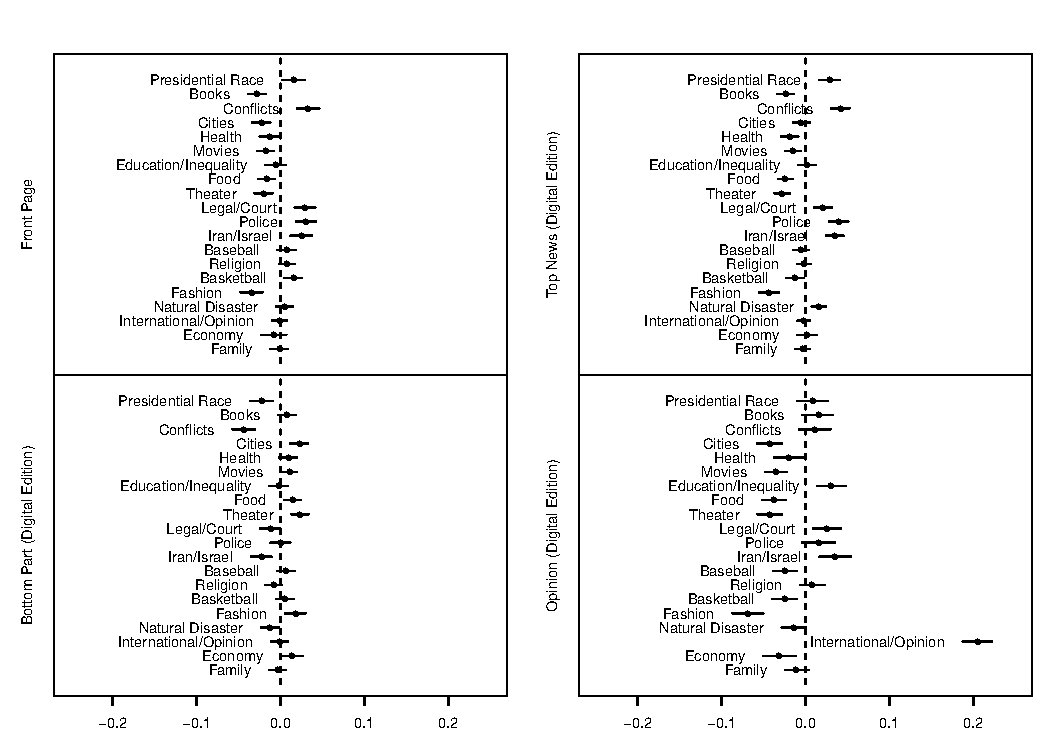
\includegraphics[width=\textwidth]{../calc/fig/res_nyt}
\end{figure}

\begin{figure}[h]
\caption{Differences between categories}\label{fig:res_share}
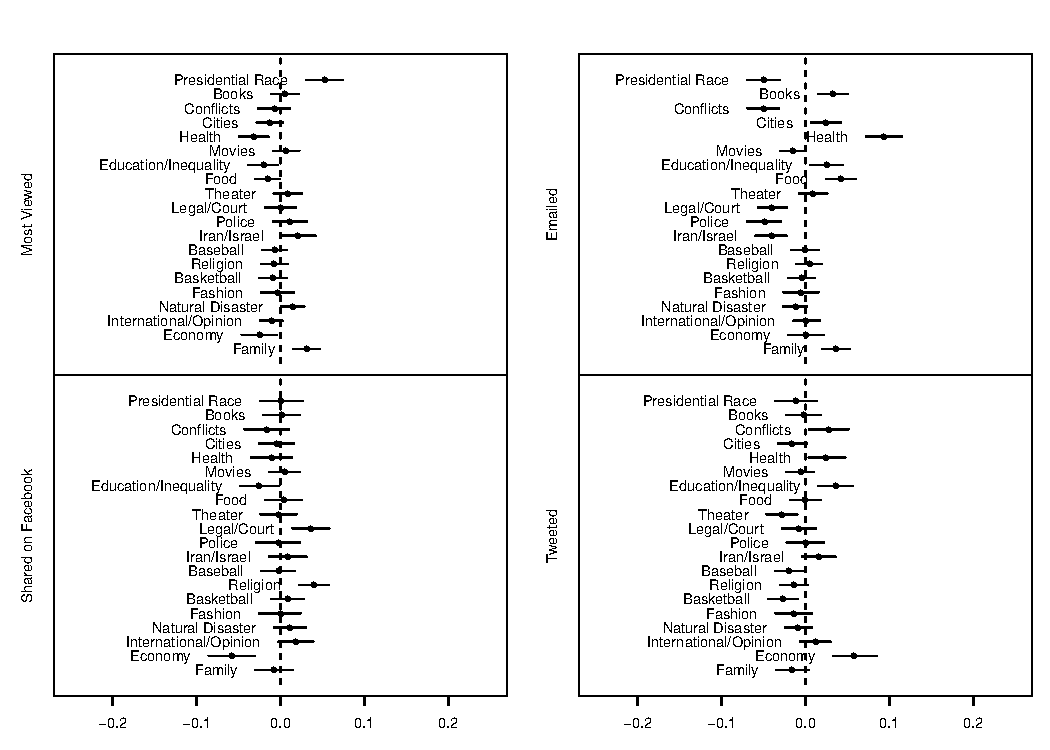
\includegraphics[width=\textwidth]{../calc/fig/res_share}
\end{figure}


\clearpage
\section{Topic proportions over time (all topics)}\label{app:series}
\renewcommand\thefigure{\thesection.\arabic{figure}}
\renewcommand\thetable{\thesection.\arabic{table}}
\setcounter{figure}{0}
\setcounter{table}{0}

\begin{figure}[h]
\caption{Topic proportions over time}\label{fig:series_nyt}
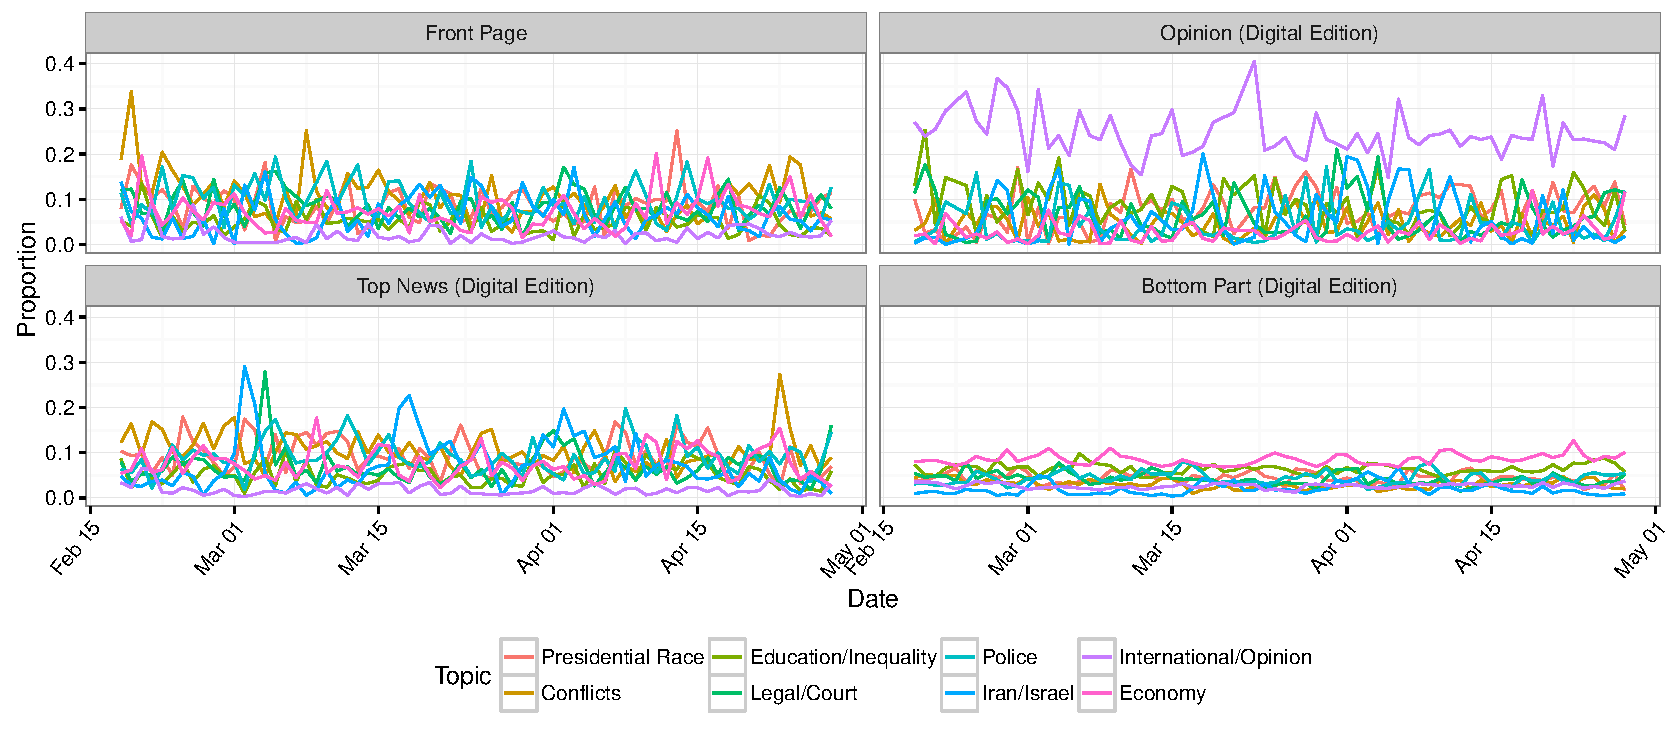
\includegraphics[width=\textwidth]{../calc/fig/series_nyt}
\end{figure}

\begin{figure}[h]
\caption{Topic proportions over time}\label{fig:series_share}
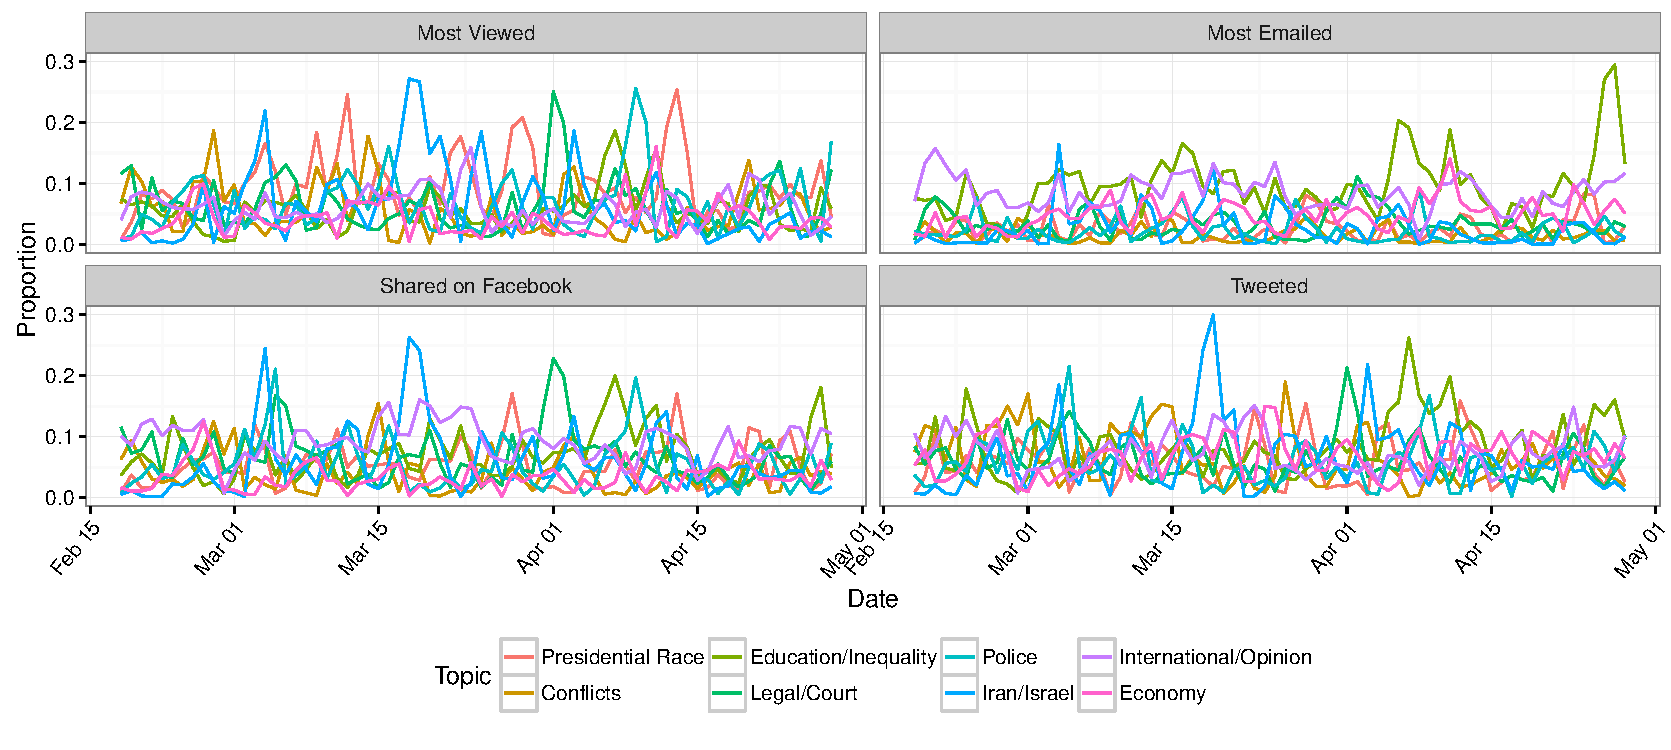
\includegraphics[width=\textwidth]{../calc/fig/series_share}
\end{figure}



\end{document} 